\documentclass[11pt]{article}
\usepackage[hmargin=1in,vmargin=0.85in]{geometry}
\usepackage[utf8]{inputenc}
\usepackage[T1]{fontenc}
\usepackage{times}
\usepackage{microtype}
\usepackage{amsmath,amssymb}
\usepackage{booktabs}
\usepackage{graphicx}
\usepackage{xcolor}
\usepackage[numbers,sort&compress]{natbib}
\usepackage[colorlinks=true,linkcolor=blue!60!black,citecolor=blue!60!black,urlcolor=blue!60!black]{hyperref}
\usepackage[capitalize,noabbrev]{cleveref}

\newcommand{\holdoutN}{30}
\newcommand{\fitN}{12}
\newcommand{\nCalls}{1{,}276}
\newcommand{\totalTokens}{157{,}132}
\newcommand{\elapsedMinutes}{21.3}
\newcommand{\noWitnessUpper}{9.5}
\newcommand{\oldOn}{3.46}
\newcommand{\oldOff}{5.21}
\newcommand{\unboundCorrect}{11}
\newcommand{\strictPrimary}{1}
\newcommand{\strictSecondary}{0}
\newcommand{\primaryFull}{28}
\newcommand{\primaryNew}{87}
\newcommand{\controlNew}{87}
\newcommand{\newTotal}{90}
\newcommand{\primaryRatio}{0.54 [0.40, 0.69]}
\newcommand{\primaryDelta}{-0.11 [-0.34, 0.11]}
\newcommand{\primaryAbs}{0.48 [0.35, 0.64]}
\newcommand{\primaryPairAbs}{0.90 [0.73, 1.06]}
\newcommand{\primaryFullChange}{-0.63 [-1.02, -0.27]}
\newcommand{\primaryCountThird}{0.47}
\newcommand{\primaryPredChange}{+0.28}
\newcommand{\primaryResidualGap}{-0.24 [-0.54, 0.00]}
\newcommand{\secondaryResidualGap}{-0.18 [-0.46, 0.08]}
\newcommand{\primaryCountError}{1.09 [0.80, 1.42]}
\newcommand{\primaryPairError}{0.48 [0.35, 0.64]}
\newcommand{\primaryCorrectedError}{0.69 [0.52, 0.88]}
\newcommand{\primaryTokens}{124}
\newcommand{\secondaryTokens}{122}
\newcommand{\witnessSeed}{101}
\newcommand{\witnessMargin}{-0.60}
\newcommand{\witnessProper}{0.20}
\newcommand{\witnessReworded}{+0.06}
\newcommand{\witnessPair}{+0.95}
\newcommand{\witnessCount}{+3.48}
\newcommand{\witnessCorrected}{+0.83}
\newcommand{\witnessRival}{3}

\title{\textbf{A Wording-Sensitive Case of Three-Way Write Skew in In-Context Memory}}
\author{Manoj Bajaj}
\date{}
\hypersetup{pdftitle={A Wording-Sensitive Case of Three-Way Write Skew in In-Context Memory},pdfauthor={Manoj Bajaj}}

\begin{document}
\maketitle
\begin{abstract}
Three new rules in a prompt can flip an old decision even when every proper subset preserves it.
Such a crossing does not establish a three-way interaction: small additive losses may suffice.
We score all eight subsets of \holdoutN{} triples on frozen Qwen2.5-0.5B-Instruct, holding token length, positions, and queue labels fixed, and compare with disjoint triples and a separately fitted count curve.
One primary-query triple flips the old answer only when fully active; both a pairwise extrapolation and a count-only forecast miss it, and all three new rules remain readable.
Changing only the question wording restores the old answer in that store.
After count correction, mean three-way residual size does not distinguish the focal triples from disjoint replacements.
The experiment establishes a wording-sensitive case, not a robust retention failure that warrants escalating to weight edits.
\end{abstract}

\section{Introduction}

A store can preserve a rule's text while losing the model behavior that rule taught.
In a joint prompt, appending three entries for unrelated keys does not overwrite an old record, but it can change how the reader uses that record.
Suppose each new entry is safe alone and every pair is safe, yet the triple flips the old answer.
An audit that checks at most two entries at a time would approve that triple.
The database analogy is write skew: changes valid in isolation can violate a shared invariant when combined~\citep{berenson1995}.
Here writes are prompt entries, not concurrent transactions, and the invariant is a model prediction rather than a database constraint.

A flip is not, on its own, evidence of a three-way interaction.
Three additive losses can exhaust a margin even if no two do.
Conversely, a nonzero three-way coefficient need not cause a flip, and can arise from a nonlinear response to rule count alone.
An earlier routing probe found that many unrelated records reduce old-rule margins, but did not vary all subsets at matched token positions~\citep{cldilution,clreanalysis}.
This leaves open whether the loss needs a particular combination of lessons.

We separate these claims using a complete three-lesson factorial with a frozen reader.
All eight contexts retain the old rule, token length, positions, and printed queue labels.
We check the old answer against every rival and estimate the three-way contrast against a fixed rival.
A pairwise extrapolation tests whether lower-order evidence would already forecast the flip; a separate count fit and disjoint replacement triples test whether the remaining variation is distinctive.
In \holdoutN{} held-out stores, we find one case that both forecasts miss; it vanishes under a second phrasing (\cref{fig:factorial}).
The goal is a screening decision on this setting, not an estimate of write skew across learners.

\begin{figure}[t]
\centering
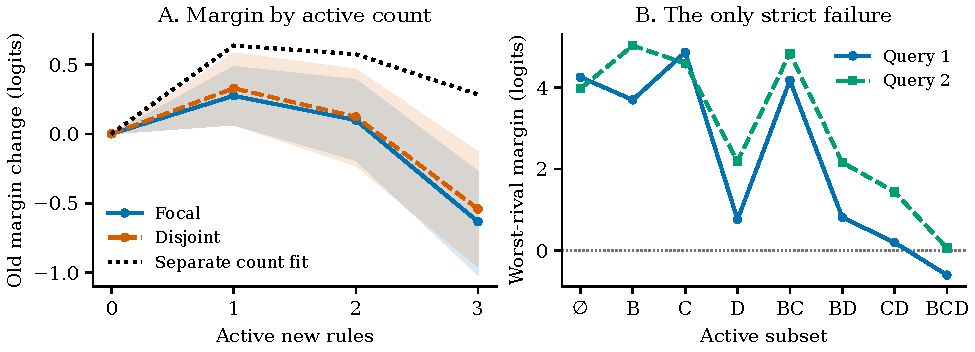
\includegraphics[width=\linewidth]{factorial.pdf}
\caption{\textbf{The only strict failure depends on the wording of the query.}
Left: mean change from the no-new-rule cell in the fixed-rival margin by active rule count.
Points average the available subsets within each of \holdoutN{} held-out stores; bands are store-bootstrap 95\% intervals.
The count fit uses \fitN{} separate stores.
Right: each point is the worst-rival margin for one subset of the sole strict witness (store \witnessSeed{}).
Below zero the old rule is no longer the top prediction. Query 2 keeps the identical store and changes only the question wording.}
\label{fig:factorial}
\end{figure}

\section{Protocol}
\label{sec:protocol}

\paragraph{Fixed slots.}
The reader is Qwen2.5-0.5B-Instruct in FP16~\citep{qwen2024}.
Each store has one fixed old routing rule, \texttt{kavimer} $\mapsto 4$, and three slots containing candidate rules $B,C,D$ for distinct, unrelated ticket types.
The candidates map to different non-target queues; the control triple changes only keys, not queues or slots.
For a subset $S\subseteq T=\{B,C,D\}$, slots outside $S$ use token-matched notes.
Notes preserve each slot's printed queue and are marked as inactive in the instruction.
Each prompt asks one of two questions about the old key.
The old slot is drawn once per store, not per subset.
We verify token length and the positions of the old rule and query in every old-read prompt.

\paragraph{Retention and three-way interaction.}
Let $m_r(S)$ be the logit for queue 4 minus the logit for rival queue $r$ in subset $S$.
A strict failure requires $\min_{r\neq4}m_r(S)>0$ for every proper subset and $\min_{r\neq4}m_r(T)\leq0$.
For a continuous contrast, pick the strongest rival at $S=\varnothing$ and freeze it for both cubes in a store and wording.
Write $m(S)$ for that fixed-rival margin.
The prediction from all lower-order coefficients and its error are
\begin{align}
\widehat m_2(T) &= \sum_{|S|=2}m(S)-\sum_{|S|=1}m(S)+m(\varnothing), \\
\Delta_3 &= m(T)-\widehat m_2(T).
\end{align}
The contrast is the third finite difference on the Boolean cube.
The pair effects for two entries $i,j$ are $m(ij)-m(i)-m(j)+m(\varnothing)$, where $m(ij)$ is shorthand for $m(\{i,j\})$.
We divide the mean $|\Delta_3|$ by the mean absolute pair effect, averaging over stores and pairs.
We use all five rival-specific predictions, not just the fixed rival, when counting missed flips.

\paragraph{Count controls.}
In each of \fitN{} separate stores we average the margin changes from $m(\varnothing)$ within each active count $k$.
Let $g(k)$ be the mean of those averages across fit stores.
The count-only prediction for a held-out store is $m(\varnothing)+g(3)$; its generic three-way component is
$g(3)-3g(2)+3g(1)-g(0)$.
We also add this component to the pairwise forecast to test whether generic curvature improves it.
For predicted flips, we fit the same curve separately for each of the five rivals rather than using the fixed-rival aggregate curve.
Neither count fit uses nonempty held-out cells.
The disjoint triple tests the typical variation from another set of random keys with the same syntax and position, not a different key population.
We resample paired stores for 95\% bootstrap intervals, conditional on the count fit; masks, rivals, and wordings are not independent replicates.

\paragraph{Screen.}
The earlier proposal set a relative interaction floor of $0.10$.
A contrast above that floor does not suffice: promotion also requires a strict failure missed by the lower-order forecast and evidence beyond count curvature or generic matched fillers.
This test neither trains weights nor selects candidate keys based on model scores.

\section{Results}
\label{sec:results}

\paragraph{Checks.}
The analyzer recovers zero three-way contrast for an additive threshold crossing,
recovers the count contrast for a count-only crossing, and detects a planted triple-only crossing that the pairwise forecast misses.
On the token-matched calibration prompt, merely marking the old record as a note kept the answer correct and increased its margin from \oldOn{} to \oldOff{} logits.
Thus the marker alone is not proof that the reader ignores inactive text.
In a post hoc check at zero active new rules, replacing the old record with a disjoint note of the same token length and queue dropped old-key accuracy from \holdoutN/\holdoutN{} to \unboundCorrect/\holdoutN{}.
With all three writes active, the model reads \primaryNew/\newTotal{} focal new keys and \controlNew/\newTotal{} disjoint new keys correctly on their own probes.

\paragraph{One strict witness.}
The primary query fails only at the full triple in \strictPrimary{} focal store (\cref{tab:retention}).
Its lowest proper-subset margin is \witnessProper{} logits, but the full-set margin against the winning queue (\witnessRival{}) is $\witnessMargin{}$ logits.
The pair-only, count-only, and curvature-corrected pair forecasts predict worst-rival margins of
$\witnessPair{}$, $\witnessCount{}$, and $\witnessCorrected{}$ respectively.
All three new rules remain correct on their own queries in this store.
The original runner-up is not the rival that wins at the full set.
With query 2, the same store stays correct at every subset, including the full set ($\witnessReworded{}$ logits; \cref{fig:factorial}).
No focal store is a strict witness under query 2; its one-sided 95\% upper bound is \noWitnessUpper\% for this store sampler.

\paragraph{The aggregate contrast does not distinguish the focal triples.}
Primary-query focal trials pass the magnitude floor: the ratio of mean absolute third difference to mean absolute pair effect is \primaryRatio{} (95\% interval).
The separately fit count curve predicts a full-set gain of $\primaryPredChange{}$ logits, not the observed mean shift of \primaryFullChange{} logits.
Adding its curvature does not improve the pairwise forecasts in this run (\cref{tab:predictions}).
Yet the disjoint controls are at least as variable by point estimate: the focal-minus-disjoint mean absolute count-centered contrast is \primaryResidualGap{} logits for query 1 and \secondaryResidualGap{} for query 2.
Neither interval establishes larger focal residuals.

\begin{table}[t]
\centering
\caption{\textbf{Retention is checked against every rival, not just the original runner-up.}
Each row covers \holdoutN{} held-out stores. \emph{Strict} counts cubes where every proper subset is correct but the full triple is not.
\emph{Misses} count strict failures the corresponding forecast predicts to be safe.
Token count is per old-read prompt, including the fixed cue.}
\label{tab:retention}
\begin{tabular}{llrrrrrr}
\toprule
& & \multicolumn{2}{c}{Old correct} & & \multicolumn{2}{c}{Misses} & \\
\cmidrule(lr){3-4}\cmidrule(lr){6-7}
Query & Triple & Empty & Full & Strict & Pair & Pair + count & Tokens \\
\midrule
\csname @@input\endcsname table_retention.tex
\bottomrule
\end{tabular}
\end{table}

\begin{table}[t]
\centering
\caption{\textbf{Forecast error quantifies departures from each control.}
Mean absolute error (MAE, logits, lower is better) measures forecast accuracy on the full-triple fixed-rival margin.
\emph{Ratio} is mean absolute cubic over mean absolute pair effect.
Ranges are store-bootstrap 95\% intervals conditional on the count fit.}
\label{tab:predictions}
\small
\setlength{\tabcolsep}{4pt}
\begin{tabular}{llrrrr}
\toprule
& & \multicolumn{3}{c}{Full-triple MAE} & \\
\cmidrule(lr){3-5}
Query & Triple & Count & Pair & Pair + count & Ratio \\
\midrule
\csname @@input\endcsname table_predictions.tex
\bottomrule
\end{tabular}
\end{table}

The factorial run takes \elapsedMinutes{} minutes on CPU with \nCalls{} scoring requests and \totalTokens{} logical input tokens, including calibration and full-store checks of the new keys.
The focal and disjoint arms use the same prompt budget and checkpoint (\cref{tab:retention}).

\section{Discussion}

\paragraph{Screening decision.}
A store can produce a three-way decision failure missed by its measured lower orders.
In this test the failure survives count correction but not a question rephrasing, and third-order residual size does not separate the two matched sets.
We retain the factorial test as a diagnostic and do not promote the write-skew idea to a weight-edit experiment on this evidence.
Count alone is not an adequate predictor here, so the decision is not a claim that all interference is additive or explained by load.

\paragraph{Related work.}
Shared prompts are known to exhibit position-dependent retrieval~\citep{liu2024} and interference across examples and tasks~\citep{rod2026,li2026}.
Prompt-composed agents can also exhibit cross-module interference without changing their final decision~\citep{lin2026}.
Those findings motivate separate tests of continuous drift and decision flips.
Our contrast asks a narrower question on synthetic routing: can the complete triple be predicted from its own smaller subsets or from the behavior of independent, same-load triples?

\paragraph{Scope.}
The independent replicates are store draws around one fixed old key, instruction, and checkpoint.
The two wordings reuse the same stores and target.
The filler arm is a second random draw from the same design, so agreement across arms cannot rule out rare or systematic interactions among a distinct family of lessons.
We test at most three active new records and do not estimate failure under long prompts, overlapping keys, multi-hop rules, or gradient updates.
The labels and templates define the task; softmax attention or other internal mechanisms are not identified by the observed contrasts.
Inactive slots are matched text, not absent model inputs; the marker control shows why that distinction matters.
An exact keyed lookup never forgets an unchanged mapping in this task. It is a semantic reference, not a measured language-model baseline.

\paragraph{Reproduction.}
The protocol, runner, verified checkpoint identifier, per-store scores, and summary are in the
\href{https://github.com/manojbajaj95/cl/tree/7932640bbf3067fd87245dbefaecef5a694e8a5b/experiments/write_skew}{experiment archive}.
The paper's tables and figures are generated from the saved results.


\begin{samepage}
\section*{AI use}
Manoj Bajaj directed the research program and commissioned this study.
Devin (Cognition AI) generated and screened the idea within that program, searched the literature, designed and ran the experiment, analyzed the data, and wrote the paper.
The paper was submitted without a separate human review of the PDF.
Qwen2.5-0.5B-Instruct supplied the experimental scores; it did not draft or review the paper.
\end{samepage}

\bibliographystyle{plainnat}
\setlength{\bibsep}{2pt}
\bibliography{references}
\appendix
\section{Implementation and calibration}
\label{app:details}

Store seeds are 0--11 for the count fit and 100--129 for the held-out test.
We sample three syllables from a fixed list of sixteen, rejecting duplicate keys and lines not matching the old rule's tokenized length.
All active and inactive entries have the same sentence shape except for the initial \texttt{Tickets} or \texttt{Notes} marker and the key.
The full prompt follows Qwen's chat markers and ends in an assistant cue, \texttt{Queue}, followed by a space.
Each candidate digit is one token following that cue.
We read six-way log probabilities with an equal logit offset on the six digits and retain exactly those six probabilities.
The offset and common normalizer cancel in pairwise log-odds.
The scorer checks the returned token identities and verifies invariance to a larger offset on the calibration prompt.

Query 1 asks where a newly arrived ticket belongs; query 2 asks which queue handles the ticket type. Both request only a number.
We use query 1 to check each new key in its fully active cube and score the shared all-inactive cell once per store and wording.
On the calibration prompt, prefix caching agrees with an uncached read within $10^{-3}$ log-probability units.
We run inference only on an eight-thread Intel Xeon CPU.

Bootstrap intervals use 10,000 resamples of the held-out store indices with replacement.
The exact one-sided zero-event upper limit, where applicable, solves $(1-p)^n=0.05$ for $n$ store draws.

\paragraph{Synthetic crossing checks.}
The additive margin $m(S)=2.5-|S|$ fails only at the full set, but its third difference is zero.
A count curve $(2.5,2,1,-1)$ also fails only at the full set and gives third difference $-0.5$ without any identity effect.
If all proper subsets instead score $1$ and the triple scores $-1$, the pair forecast is $1$ and misses by $-2$ logits (observed minus predicted).
These cubes check the analysis, not the language model.

\end{document}
